\begin{figure}[H]
\begin{center}
    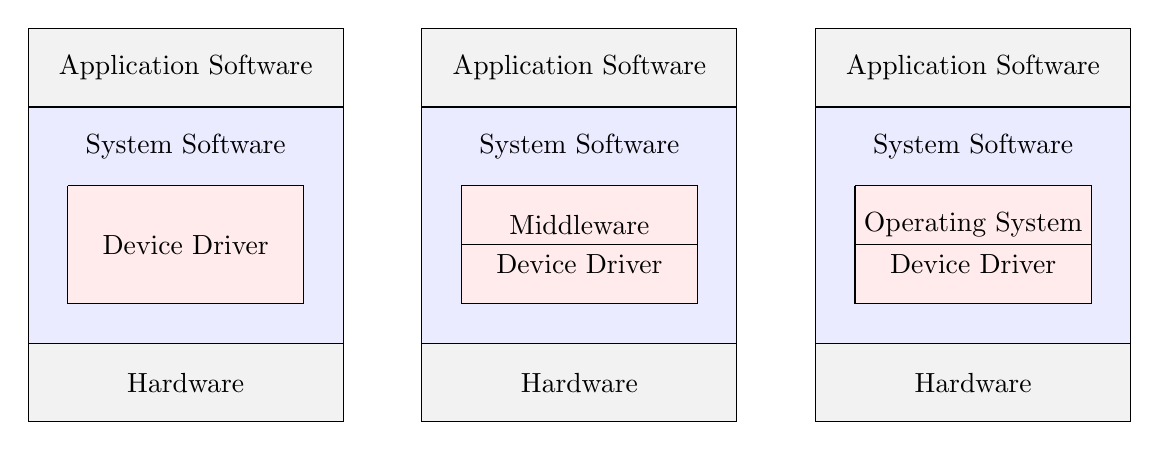
\begin{tikzpicture}
        \draw[fill=gray!10] (0,0) -- (4,0) -- (4,-5) -- (0,-5) -- (0,0);
        \draw[fill=blue!8] (0,-1) -- (4,-1) -- (4,-4) -- (0,-4) -- (0,-1);
        \draw[fill=red!8] (0.5,-2) -- (3.5,-2) -- (3.5,-3.5) -- (0.5,-3.5) -- (0.5,-2);

        \draw[fill=gray!10] (5,0) -- (9,0) -- (9,-5) -- (5,-5) -- (5,0);
        \draw[fill=blue!8] (5,-1) -- (9,-1) -- (9,-4) -- (5,-4) -- (5,-1);
        \draw[fill=red!8] (5.5,-2) -- (8.5,-2) -- (8.5,-3.5) -- (5.5,-3.5) -- (5.5,-2);
        \draw (5.5,-2.75) -- (8.5,-2.75);

        \draw[fill=gray!10] (10,0) -- (14,0) -- (14,-5) -- (10,-5) -- (10,0);
        \draw[fill=blue!8] (10,-1) -- (14,-1) -- (14,-4) -- (10,-4) -- (10,-1);
        \draw[fill=red!8] (10.5,-2) -- (13.5,-2) -- (13.5,-3.5) -- (10.5,-3.5) -- (10.5,-2);
        \draw (10.5,-2.75) -- (13.5,-2.75);

        \draw (2,-0.5) node[] {Application Software};
        \draw (2,-1.5) node[] {System Software};
        \draw (2,-2.75) node[] {Device Driver};
        \draw (2,-4.5) node[] {Hardware};
        
        \draw (7,-0.5) node[] {Application Software};
        \draw (7,-1.5) node[] {System Software};
        \draw (7,-2.5) node[] {Middleware};
        \draw (7,-3) node[] {Device Driver};
        \draw (7,-4.5) node[] {Hardware};
        
        \draw (12,-0.5) node[] {Application Software};
        \draw (12,-1.5) node[] {System Software};
        \draw (12,-2.5) node[] {Operating System};
        \draw (12,-3) node[] {Device Driver};
        \draw (12,-4.5) node[] {Hardware};
    \end{tikzpicture}
\end{center}
\caption{Embedded OSI system models}
\label{fig:embedded-osi}
\end{figure}
